
\chapter{Matrix Factorization Methods}   

This chapter covers one of the more popular RS methods, matrix
factorization.  The overall theme will be \textit{low-rank
approximation}:  given a matrix $M_1$,  find a matrix $M_2$ for which 

\begin{equation}
rk(M_2) << rk(M_1)
\end{equation}

and 

\begin{equation}
M_2 \approx M_1
\end{equation}


To set the stage, we start with a more basic matrix
operation, PCA.

\section{An Approach to Approximate Rank:  Principal Components
Analysis}

Suppose the matrix in (\ref{rankex1}) had been

\begin{equation}
\label{rankex2}  
M =
\left (
\begin{array}{rrrr}
1 & 5 & 1 & -2\\
8.02 & 2.99 & 2 & 8.2\\
9 & 8 & 3 & 6 
\end{array}
\right )
\end{equation}

Intuitively, we still might say that the rank of $M$ is
``approximately'' 2.  So row 3 still seems redundant, Let's
formalize that, leading to one of the most common techniques in
statistics/machine learning.  

\subsection{Exploiting Correlations}
\label{explorecorr}

Statistically, the issue is one of correlation.  In (\ref{rankex2}), the
third row is highly correlated with (the sum of) the first two rows.  To
explore the correlation idea further, recall our two graphs of bivariate
normal densities from Section \ref{mvnormal}:

\begin{minipage}[b]{0.65\linewidth}
    \mbox{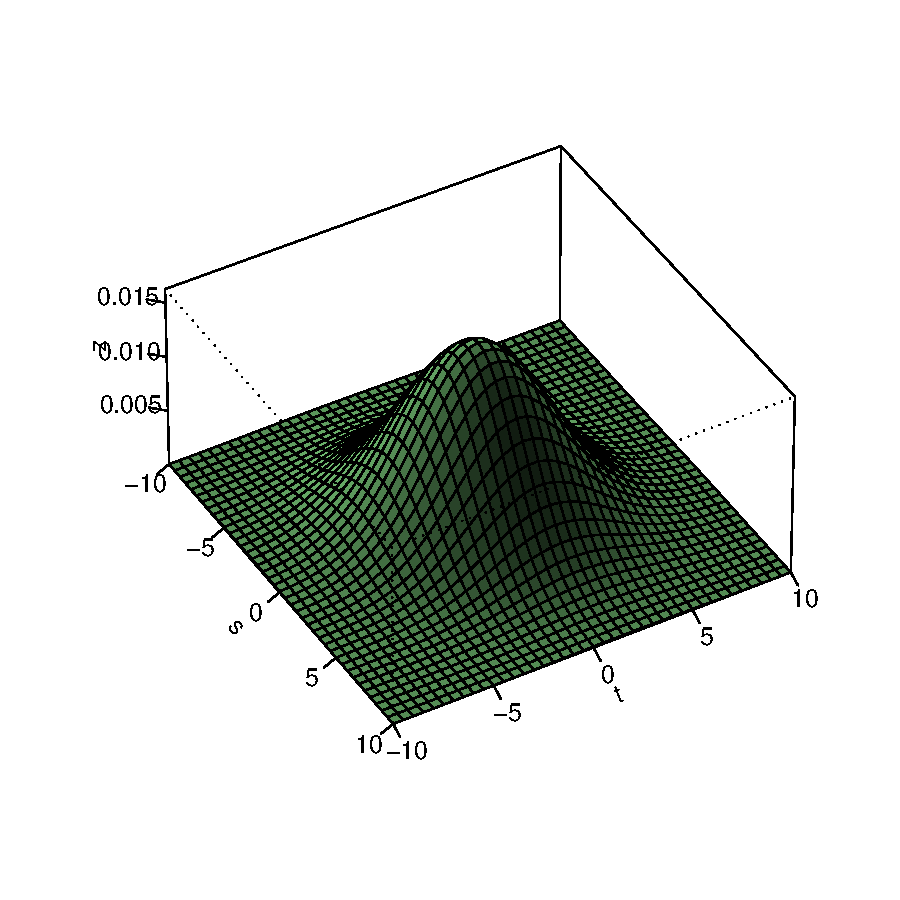
\includegraphics[width=3.25in]{Images/Rho2.pdf}} 
\end{minipage}
\hspace{0.0in}
\begin{minipage}[b]{0.65\linewidth}
    \mbox{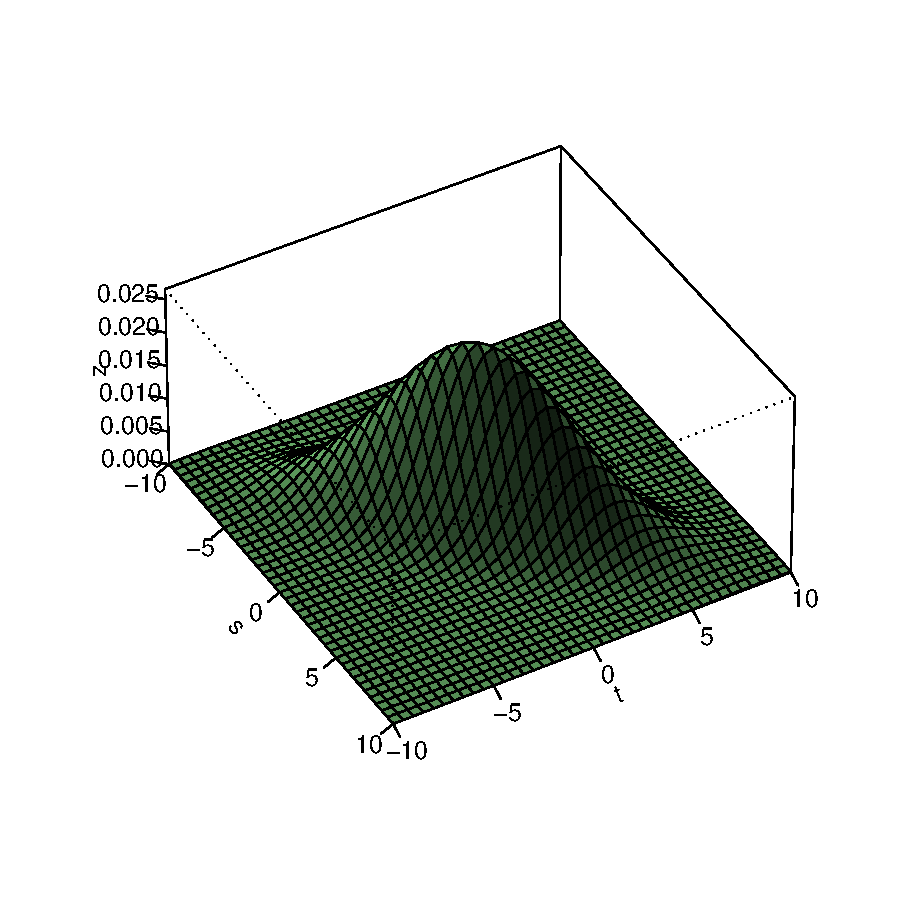
\includegraphics[width=3.25in]{Images/Rho8.pdf}} 
\end{minipage}

The two plots were for a low-correlation (0.2) distribution and a
high-correlation (0.8) one.  As we said at the time about the latter:

\begin{quote}

The probability that $X_2 \approx X_1$ is high.  So, to a large extent,
there is only one variable here, $X_1$ (or other choices, e.g.\ $X_2$),
not two.  

\end{quote}

In the case of correlation 0.2, the two variables are more separate.
The probability that $X_2 \approx -X_1$ is lower here.

Note one more time, though, the approximate nature of the approach we
are developing.  There really \textit{are} two variables even in that
correlation 0.8 example.  By using only one of them, \textbf{we are
relinquishing some information.  But with the need to avoid overfitting,
use of the approximation may be a net win for us.}

Well then, how can we determine a set of near-redundant variables, so
that we can consider omitting them from our analysis?  Let's look at
those graphs a little more closely.

Any \textit{level set} in the above graphs, i.e.\ a curve one
obtains by slicing the bells parallel to the $(t_1,t_2)$ plane, can be
shown to be an ellipse.  As noted, the major axis of the ellipse will be
the line $t_1 + t_2 = 0$.  The minor axis will be the line perpendicular
to that, $t_1 - t_2 = 0$.  That suggests forming new variables,

\begin{equation}
Y_1 = X_1 + X_2 
\end{equation}

and 

\begin{equation}
Y_2 = X_1 - X_2 
\end{equation}

In fact, taking

\begin{equation}
A = 
\left (
\begin{array}{rr}
1 & 1 \\
1 & -1 \\
\end{array}
\right )
\end{equation}

in (\ref{covax}) shows that $\rho(Y_1,Y_2) = 0$.

Here is the point so far:

\begin{itemize}

\item The high value of $\rho(X_1,X_2)$ suggests that for this dataset,
``one variable is enough.''  Thus we might consider using just $X_1$
rather than $X_1$ and $X_2$.

\item Or, we might consider using $Y_1$ for our one
variable.  

\end{itemize} 

Now suppose we have $p$ variables, $X_1,
X_2,...,X_p$, not just two.  If our data is on people, these variables
may be height, weight, age, gender and so on.  We can no longer
visualize in higher dimensions, but one can show that the level sets
will be $p$-dimensional ellipsoids.  These now have $p$ axes rather than
just two, and we can define $p$ new variables, $Y_1,Y_2,...,Y_p$ from
the $X_i$, such that:

\begin{itemize}

\item [(a)] The $Y_i$ are uncorrelated.

\item [(b)] They are ordered in terms of variance:

\begin{equation}
Var(Y_1) > Var(Y_2) > ... > Var(Y_p)
\end{equation}

\end{itemize} 

Now we have a promising solution to our dimension reduction problem.  In
(b) above, we can choose to use just the first few of the $Y_i$,
omitting the ones with small variance since they are essentially
constants, uninformative.  And again, since the $Y_i$ will be
uncorrelated, we are eliminating a source of possible redundancy among
them; after all, we are doing dimension reduction, i.e.\ we wish to
reduce the number of variables, so we don't want any redundant ones.

PCA won't be a perfect solution --- there is no such thing --- as might
be the case if the relations between variables is nonmonotonic.  A
common example is age and income, with mean income given age tending to be a
quadratic (or higher degree) polynomial relation.  But PCA is a very
common ``go to'' method for dimension reduction, and may work well even
in (mildly) nonmonotonic settings.

Note too that although we've motivated things here with multivariate
normal distributions, we haven't assumed it.  We are merely talking
about finding a set of uncorrelated variables that are linear functions
of our original ones.

Now, how do we find these $Y_i$?

\subsection{Eigenanalysis}

Say we have a sample of $n$ observations on $p$ variables, say $p$
measurements on each of $n$ people.  The measurements are $X_1,...,X_p$.
For example, we might have $p=3$, with $X_1, ~ X_2, \textrm{ and } X_3$
being height, weight and age.  

% Let $X_{ik}$ be the value of $X_i$ on the $k^{th}$ person, $k = 1,...,n$.
% 
% The sample correlation between $X_i$ and $X_j$ is the sample
% analog of (\ref{rhodef}),
% 
% \begin{equation}
% \label{corrdef}
% \widehat{\rho} =
% \frac
% {\frac{1}{n} \sum_{k=1}^n (X_{ik}-\overline{X}_i)
% (X_{jk}-\overline{X}_j)}
% {s.d.(X_i) ~ s.d.(X_j)}
% \end{equation}
% 
% where the denominator is the product of the sample standard deviations
% of the two variables, and $\overline{X}_i)$ and $\overline{X}_j)$ are
% the sample means.  

Let $C$ denote the covariance matrix of $X_1,...,X_p$.  Note that
since $Cov(X_i,X_j) = Cov(X_j,X_i)$, 
the matrix $C$ is \emph{symmetric},

\begin{equation}
C' = C
\end{equation}

Recall that for any square matrix $L$, if there is a scalar $\lambda$
and a nonzero vector $x$ such that 

\begin{equation}
Lx = \lambda x
\end{equation}

then we say that $x$ is an \textit{eigenvector} of $L$, with
\textit{eigenvalue} $\lambda$.  

It can be shown\footnote{Here and below, ``can be shown'' means that the
assertion is proved in any standard textbook on linear algebra.} that
any symmetric matrix has real (not complex) eigenvalues, and that the
corresponding eigenvectors $U_1,...,U_p$ are \textit{orthogonal},

\begin{equation}
U_i' U_j = 0, ~ i \neq j
\end{equation}

We always take the $U_i$ to have length 1:  Just divide the vector by
its length, so it now has length 1, and is still an eigenvector.  

Let $U$ denote the $p \times p$ matrix whose $i^{th}$ column is $U_i$.
then from the orthogonality of the eigenvectors, we have

\begin{equation}
\label{uui}
U'U = I
\end{equation}

the $p \times p$ identity matrix.  We also refer to $U$ as
\emph{orthogonal}.

It also can be shown that 

\begin{equation}
UCU' = D
\end{equation}

where $D$ is a diagonal matrix with the eigenvalues of $C$ on the
diagonal.

Multiplying on the left by $U'$ and the on the right by $U$,
and using (\ref{uui}), we have

\begin{equation}
C = U'DU
\end{equation}

Now, form a new random vector from the random vector 
$X = (X_1,...,X_p)'$:

\begin{equation}
Y = U'X
\end{equation}$

Let's find its covariance matrix, again using (\ref{covax}):

\begin{equation}
Cov(Y) = U
\end{equation}

\subsection{PCA}

Typically we have many cases in our data, say $n$, arranged in an $n
\times p$ matrix $Q$, with row $i$ representing case $i$ and column $j$
representing the $j^{th}$ variable.

Say our data is about people, 1000 of them, and we have data on height,
weight, age, gender, years of schooling and income.  Then $n = 1000$, $p
= 6$.

So, finally, here is PCA:

\begin{enumerate}


\item Find the correlation matrix (or covariance matrix)
from the data in $Q$.  Note again that since there are $p$
variables, the correlation matrix will be $p \times p$.

\item Compute its eigenvalues and eigenvectors.  It can be shown that
the eigenvalues are the variances of our new variables.

\item After ordering the eigenvalues from largest to smallest, let
$\lambda_i$ be the $i^{th}$ largest, and let $U_i$ be the corresponding
eigenvector, scaled to have length 1.  

\item Let $U$ be the matrix whose $i^{th}$ column is $U_i$.  Its size
will be $p \times p$.

\item Choose the first few eigenvalues, say $s$ of them, using some
criterion (see below).  Denote the matrix of the first $s$ columns of $U$
by $U^{(s)}$.  

\item Form a new data matrix, 

\begin{equation}
\label{rqu}
R = Q U^{(s)}
\end{equation}

$R$ will be of size $n \times s$.  So, we've replaced our original $p$
variables, the $p$ columns of $Q$, by $s$ new variables, the columns of
$R$.  Column $j$ of $R$ is called the $j^{th}$ principal component of
the original data.  

As mentioned, it can be shown that the variance of the $j^{th}$ principal
component is $\lambda_j$.  The sum of all $p$ eigenvalues is the same as
the sum of the variances of the original variables, an important point.

\end{enumerate} 

From this point onward, any data analysis we do will be with $R$, not
$Q$.  In $R$, row $i$ is still data on the $i^{th}$ case, e.g. the
$i^{th}$ person, but now with $s$ new variables in place of the original
$p$.  Since typically $s << p$, we have achieved considerable dimension
reduction.

\subsection{Applying Matrix Partitioning}

Using the approach of Section \ref{partmat}, partition $U^{(s)}$ into
its columns,

\begin{equation}
U^{(s)} = (U_1,...,U_s) 
\end{equation}

and thus write

\begin{equation}
\label{rqu1}
R = Q U^{(s)} = Q (U_1,...,U_s)
\end{equation} 

After that second equality, pretend that $Q$ and the $U_i$ are
``numbers.''  Then the last expression in (\ref{rqu1}),

\begin{equation}
Q (U_1,...,U_s)
\end{equation}

is a ``scalar'' times a ``vector,'' and is thus equal to 

\begin{equation}
(QU_1,...,QU_s)
\end{equation}

So, the $i^{th}$ column of $R$ is $Q U_i$.  The latter quantity is of
the $Ax$, matrix-times-vector form of Section \ref{mfact}, so it is a
linear combination of the columns of $Q$, with the coefficients in that
linear combination being the elements in $U_i$.  

Recall that each column of $Q$ is one variable; e.g.\ for people, there
may be an age column, a height column, a weight column and so on.  Each
column in $R$ is one of our new variables.  Therefore:

\begin{quote}
The $i^{th}$ new variable is equal to a linear combination of the old
variables.
\end{quote}

So, a new variable might be, say, 1.9 age + 0.3 height + 1.2 weight.

% \subsection{Why It Works}
% 
% Recall that the new variables have the $\lambda_i$ for variances and are
% uncorrelated.  Here's why:
% 
% It is common (especially in neural networks, by the way) to
% \textit{center} and \textbf{scale} one's data, meaning to subtract from
% each variable its mean, and divide by its standard deviation.  For
% instance, if one variable is human height and its standard deviation is
% 3.2 inches, we divide the height column in $Q$ by 3.2 (after subtracting
% mean height).
% 
% The new mean and standard deviation are 0 and 1.  In that case,
% (\ref{corrdef}) becomes
% 
% 
% \begin{equation}
% \frac{1}{n} \sum_{i=1}^n x_i y_i
% \end{equation}
% 
% Using this insight, the reader should verify that with the matrices $Q$
% and $R$ above (old and new data), their correlation matrices are $Q'Q$
% and $R'R$.  Let's see how that works out:
% 
% \begin{eqnarray}
% \label{rrqq}
% R'R &=& (Q U^{(s)})' (QU^{(s)}) \\  
% &=&  
% U^{(s)} {}' Q' ~ Q U^{(s)} \\
% \end{eqnarray}
% 
% using the fact that $(AB)' = B'A'$.
% 
% But remember that the $U_i$ are eigenvectors of the correlation matrix,
% in this case $Q'Q$!  So
% 
% \begin{equation}
% \label{qqu}
% (Q'Q) U^{(s)} = (Q'Q) (U_1,U_2,...,U_s) = 
% (\lambda_1 U_1,...,\lambda_s U_s)
% \end{equation}
% 
% Finally, recall that the $U_i$ are orthogonal with length 1.
% Substituting (\ref{qqu}) in (\ref{rrqq})e then get
% 
% \begin{equation}
% R'R = U^{(s)}'(Q'Q) U^{(s)} =
% U^{(s)}'(\lambda_1 U_1,...,\lambda_s U_s)
% = \textrm{diag}(\lambda_1,...,\lambda_s)
% \end{equation} 
% 
% the matrix having the $\lambda_i$ on the diagonal and 0s elsewhere.  The
% latter imply that the new variables are uncorrelated, and the former
% fact says that the variances of the new variables are the $\lambda_i$,
% as claimed.

\subsection{Choosing the Number of Principal Components}  

The number of components we use, $s$, is called a \textit{tuning
parameter} or \textit{hyperparameter}.  So, how do we choose $s$?  This
is the hard part, and there is no universal good method.  Typically $s$
is chosen so that 

\begin{equation} 
\sum_{j=1}^s \lambda_j
\end{equation}

is ``most'' of total variance (again, that total is the above expression
with $p$ instead of $s$), but even this is usually done informally.

In ML/RS settings, though, $s$ is typically chosen by a technique called
\textit{cross validation}, to be discussed in Chapter \ref{chap:infra2}.

\subsection{Software and UCI Repository Example}

The most commonly used R function for PCA is \textbf{prcomp()}.  As with
many R functions, it has many optional arguments; we'll take the default
values here.

For our example, let's use the Turkish Teaching Evaluation data,
available from the UC Irvine Machine Learning Data Repository.  It
consists of 5820 student evaluations of university instructors.  Each
student evaluation consists of answers to 28 questions, each calling for
a rating of 1-5, plus some other variables we won't consider here.

\begin{lstlisting}
> turk <- read.csv('turkiye-student-evaluation.csv',header=T)
> head(turk)
  instr class nb.repeat attendance difficulty Q1 Q2 Q3 Q4
1     1     2         1          0          4  3  3  3  3
2     1     2         1          1          3  3  3  3  3
3     1     2         1          2          4  5  5  5  5
4     1     2         1          1          3  3  3  3  3
5     1     2         1          0          1  1  1  1  1
6     1     2         1          3          3  4  4  4  4
  Q5 Q6 Q7 Q8 Q9 Q10 Q11 Q12 Q13 Q14 Q15 Q16 Q17 Q18 Q19
1  3  3  3  3  3   3   3   3   3   3   3   3   3   3   3
2  3  3  3  3  3   3   3   3   3   3   3   3   3   3   3
3  5  5  5  5  5   5   5   5   5   5   5   5   5   5   5
4  3  3  3  3  3   3   3   3   3   3   3   3   3   3   3
5  1  1  1  1  1   1   1   1   1   1   1   1   1   1   1
6  4  4  4  4  4   4   4   4   4   4   4   4   4   4   4
  Q20 Q21 Q22 Q23 Q24 Q25 Q26 Q27 Q28
1   3   3   3   3   3   3   3   3   3
2   3   3   3   3   3   3   3   3   3
3   5   5   5   5   5   5   5   5   5
4   3   3   3   3   3   3   3   3   3
5   1   1   1   1   1   1   1   1   1
6   4   4   4   4   4   4   4   4   4
> tpca <- prcomp(turk[,-(1:5)]
\end{lstlisting}

Let's explore the output.  First, the standard deviations of the new
variables:

\begin{lstlisting}
> tpca$sdev
 [1] 6.1294752 1.4366581 0.8169210 0.7663429 0.6881709
 [6] 0.6528149 0.5776757 0.5460676 0.5270327 0.4827412
[11] 0.4776421 0.4714887 0.4449105 0.4364215 0.4327540
[16] 0.4236855 0.4182859 0.4053242 0.3937768 0.3895587
[21] 0.3707312 0.3674430 0.3618074 0.3527829 0.3379096
[26] 0.3312691 0.2979928 0.2888057
> tmp <- cumsum(tpca$sdev^2)
> tmp / tmp[28]
 [1] 0.8219815 0.8671382 0.8817389 0.8945877 0.9049489
 [6] 0.9142727 0.9215737 0.9280977 0.9341747 0.9392732
[11] 0.9442646 0.9491282 0.9534589 0.9576259 0.9617232
[16] 0.9656506 0.9694785 0.9730729 0.9764653 0.9797855
[21] 0.9827925 0.9857464 0.9886104 0.9913333 0.9938314
[26] 0.9962324 0.9981752 1.0000000
\end{lstlisting}

This is striking.  The first principal component (PC) already accounts
for 82\% of the total variance among all 28 questions.  The first five
PCs cover over 90\%.  This suggests that the designer of the evaluation
survey could have written a much more concise survey instrument with
almost the same utility.

Now keep in mind that each PC here is essentially a ``super-question''
capturing student opinion via a weighted sum of the original 28
questions.  Let's look at the first two PCs' weights:

\begin{lstlisting}
> tpca$rotation[,1]
        Q1         Q2         Q3         Q4         Q5 
-0.1787291 -0.1869604 -0.1821853 -0.1841701 -0.1902141 
        Q6         Q7         Q8         Q9        Q10 
-0.1870812 -0.1878324 -0.1867865 -0.1823915 -0.1923626 
       Q11        Q12        Q13        Q14        Q15 
-0.1866948 -0.1862382 -0.1922729 -0.1911814 -0.1902380 
       Q16        Q17        Q18        Q19        Q20 
-0.1962885 -0.1808833 -0.1935788 -0.1927359 -0.1931985 
       Q21        Q22        Q23        Q24        Q25 
-0.1911060 -0.1908591 -0.1948393 -0.1931334 -0.1888957 
       Q26        Q27        Q28 
-0.1908694 -0.1897555 -0.1886699 
\end{lstlisting}

\begin{lstlisting}

> tpca$rotation[,2]
         Q1          Q2          Q3          Q4          Q5 
 0.35645673  0.23223504  0.11551155  0.24533527  0.20717759 
         Q6          Q7          Q8          Q9         Q10 
 0.20075314  0.24290761  0.24901577  0.12919618  0.18911720 
        Q11         Q12         Q13         Q14         Q15 
 0.11051480  0.21203229 -0.10616030 -0.15629705 -0.15533847 
        Q16         Q17         Q18         Q19         Q20 
-0.04865706 -0.26259518 -0.12905840 -0.15363392 -0.19670071 
        Q21         Q22         Q23         Q24         Q25 
-0.22007368 -0.22347198 -0.10278122 -0.06210583 -0.20787213 
        Q26         Q27         Q28 
-0.12045026 -0.07204024 -0.21401477 
\end{lstlisting}

The first PC turned out to place approximately equal weights on all 28
questions.  The second PC, though, placed its heaviest weight on Q1,
with substantially varying weights on the other questions.

While we are here, let's check that the columns of $U$ are orthogonal.

\begin{lstlisting}
> t(tpca$rotation[,1]) %*% tpca$rotation[,2]
              [,1]
[1,] -2.012279e-16
\end{lstlisting}

Yes, 0 (with roundoff error).  As an exercise in matrix partitioning,
the reader should run

\begin{lstlisting}
t(tpca$rotation) %*% tpca$rotation
\end{lstlisting}

then check that it produces the identity matrix $I$, then ponder why
this should be the case.

\subsection{MovieLens Example}

\subsection{More on the PC Coefficients}
\label{coors}

There is more to consider.

Do the PC coefficients have any interpretation?  The answer is
probably no for ordinary people, but for the \textit{domain experts},
very possibly yes.  In the teaching evaluation example above, a
specialist in survey design or teaching methods may well be able to
interpret the dominance of Q1 in the second PC.  A method called
\textit{factor analysis}, an extension of PCA, is popular in social
science research.

For the rest of us, PCA is just a handy way to do dimension reduction.

But there is geometric terminology that will be helpful, as follows.
Let's look at the \textbf{mlb} dataset from the \textbf{regtools}
package.  This is data on Major League baseball players.

\begin{lstlisting}
             Name Team       Position Height Weight   Age
1   Adam_Donachie  BAL        Catcher     74    180 22.99
2       Paul_Bako  BAL        Catcher     74    215 34.69
3 Ramon_Hernandez  BAL        Catcher     72    210 30.78
4    Kevin_Millar  BAL  First_Baseman     72    210 35.43
5     Chris_Gomez  BAL  First_Baseman     73    188 35.71
6   Brian_Roberts  BAL Second_Baseman     69    176 29.39
  PosCategory
1     Catcher
2     Catcher
3     Catcher
4   Infielder
5   Infielder
6   Infielder
\end{lstlisting}

Let's apply PCA:

\begin{lstlisting}
> hw <- as.matrix(mlb[,4:5]) 
> pcout <- prcomp(hw) 
> pcout$rotation 
               PC1         PC2
Height -0.05948695  0.99822908
Weight -0.99822908 -0.05948695
\end{lstlisting}

If we were to plot \textbf{hw}, we would put \textbf{hw[1,]} at the
point (74,180) on our graph.  Recall from high school math that 74 and
180 are called the \textit{coordinates} of \textbf{hw2[1,]}, with
respect to our ``H axis'' and ``W axis.''

But in doing PCA, we are creating new axes, PC1 and PC2, which are
rotated versions of the H and W axes.  (Hence the naming of the $U$
matrix as ``rotation'' in the \textbf{prcomp()} return value.)  Let's
find the coordinates of \textbf{hw[1,]} with respect to the new axes:

\begin{lstlisting}
> hw[1,] %*% pcout$rotation
           PC1     PC2
[1,] -184.0833 63.1613
\end{lstlisting}

So (74,180) has become (-184.1,63.2) under the new coordinate
system.  Let's see what the angle of rotation is. We can do that by
seeing where a point on the H axis rotates to.

\begin{lstlisting}
> pc10 <- c(1,0) %*% pcout$rotation
> pc10
             PC1       PC2
[1,] -0.05948695 0.9982291
> (atan(pc10[2] / pc10[1])) * 180/pi
[1] -86.58964
\end{lstlisting}

Almost 90 degrees clockwise.

\subsection{Scaling}

Some analysts prefer to \textit{scale} the data before applying PCA.
For each column, we would subtract the column mean and divide by the
column standard deviation.  The column would now have mean 0.0 and
variance 1.0.

The rationale for doing this is that if PCA is applied to the original
data, variables with large variance will dominate.  And then units would
play a role; e.g.\ a distance variable would have more impact if it were
measured in kilometers than miles.

Scaling does solve this problem, but its propriety is questionable.
Consider a setting with two features, $A$ and $B$, with variances 500
and 2, respectively, and with mean 100 for both.  Let $A'$ and $B'$
denote these features after centering and scaling.

As noted, PCA is all about removing features with small variance, as
they are essentially constant. If we work with $A$ and $B$, we would of
course use only $A$. But if we work with $A'$ and $B'$, we would use
both of them, as they both have variance 1.0.

So, dealing with the disparate-variance problem (e.g. miles vs.\
kilometers) shouldn't generally be solved by ordinary scaling, i.e.\ by
dividing by the standard deviation.  An alternative is to divide each
column by its mean.  This addresses the miles-vs.-kilometers problem,
and makes sense in that a variance is large or small in relation to its
mean.

\section{Matrix Factorization Methods}  

\section{The Setting}

Recall the brief introduction in Chapter \ref{chap:prologue}:  Let $A$
denote the ratings matrix, with the element in row $i$, column $j$
storing the rating of item $j$ given by user $i$.  Most of $A$ is
unknown, i.e.\ NA values in R.  We wish to estimate the unknown ones.

Say the dimension of $A$ is $u \times v$.  We wish to find rank-$k$
matrices $W$ ($u \times k$) and $H$ ($k \times v$) such that  

\begin{equation}
\label{awh}
A \approx W H
\end{equation}

Note that the $W$ and $H$ that we find will be \textit{fully known},
with values that will be derived somehow from the known elements of $A$.

Again, most of the elements of $A$ are unknown.  But it is typically the
case that similar users have similar ratings patterns, and the matrix
factorization will hopefully exploit that.  We thus hope to obtain good
estimates of all of $A$ even though only a small part of it is known.  

\textbf{Note that k is a tuning parameter, chosen by the user.}  One
might use cross-validation in making this choice, comparing performance
of various values of $k$.

\textit{This is a form of dimension reduction}, with the rank $k$
controlling the bias-variance tradeoff.  Typically a good approximation
can be achieved with

\begin{equation}
k \ll \textrm{ rank}(A)
\end{equation}

\section{Finding W and H}

There are two main approaches to matrix factorization in recommender
systems and general machine learning:

\begin{itemize}

\item Singular Value Decomposition (SVD):  This is a ``cousin'' of PCA,
kind of a ``square root'' of the latter.  There is a function in base R
for this, \textbf{svd()}.

\item Nonnegative Matrix Factorization (NMF): Here the matrix $A$ has
nonnegative elements, and one desires the same property for $W$ and $H$.
This may lead to sparsity in $WH$, and in some cases a helpful
intepretability.  There are several R packages for this; see below.

\end{itemize} 

Since most of the issues are the same for both methods, we'll mainly stick
to one, NMF.

\section{Notation}

We'll use the following notation for a matrix $Q$

\begin{itemize}

\item $Q_{ij}$:  element in row $i$, column $j$

\item $Q_{i \cdot}$:  row $i$

\item $Q_{\cdot j}$:  column $j$

\end{itemize}

\section{Synthetic, Representative Recommender Systems Users}
\label{synth}

Note the key relation, which we showed in Section \ref{partmat}:

\begin{equation}
(WH)_{i \cdot} = \sum_{m=1}^k W_{im} H_{m \cdot}
\end{equation}

In other words, in (\ref{awh}), we have that:

\begin{itemize}

\item The entire vector of predicted ratings by user $i$ can be
expressed as a linear combination of the rows of $H$.


\item The rows of $H$ can thus be thought of as synthetic
``users'' who are representative of users in general.  $H_{rs}$ is the
rating that synthetic user $r$ gives item $s$.

\end{itemize} 

In this manner, we can predict ratings for any user that is already in
$A$.  but what about an entirely new user?  What we need is the
coordinates of this new user with respect to the rows of $H$.  We'll see
how to get these later in the chapter.\footnote{After accumlating enough
new users, of course, we should update $A$, and thus $W$ and $H$.}

Of course, interchanging the roles of rows and columns above, we have
that the columns of $W$ serve as an approximate basis for the columns of
$A$.  In other words, the latter become synthetic, representative items,
e.g.\ representative movies in the MovieLens data.

\section{Vector Space View}

Recall that the \textit{span} of a set of vectors in a vector space is
the set of all linear combinations of those vectors.  The term
\textit{basis} in means a linearly independent set of vectors that spans
the given subspace, i.e.\ any vector in the subspace can be expressed as
a linear combinations of the basis vectors.

Thus the rows of $H$ can be thought of as an ``approximate
basis'' for the span of the rows of $A$.

\section{The Case of Entirely Known A}

In RS applications, the matrix $A$ is only partially known.  But it will
be easier to understand the methods for finding the $W$ and $H$ matrices
by looking at another class of applications.  In fact, NMF has become
widely used in a variety of ML applications in which the matrix $A$
entirely known. 

\subsection{Image Classification}
:
\textbf{The setting:}

Say we have $n$ image files, each of which has brightness data for $r$
rows and $c$ columns of pixels.  We also know the class, i.e.\ the
subject, of each image.  The famous MNIST dataset, for instance,
consists of 70,000 28x28 images of hand-drawn digits; here $n = 70000$
and $r = c = 28$.  Thus the data for an image consists of $28^2 = 784$
pixel intensities, each in the range 0,1,2,...,255.  (255 is fully
black, 0 is fully white and the others are shades of gray.) We have 10
classes, '0' through '9'.

We wish to predict the classes of new images. Denote the class of
image $j$ in our original data by $C_j$.

We form a matrix $A$ with $n$ rows and $w = rc$ columns, where the
$i^{th}$ row, $A_{i \cdot}$ stores the data for the $i^{th}$ image, say
in row-major order:\footnote{Make sure not to confuse the rows of $A$
with the rows of an image.  One row of $A$ contains the totality of rows
and columns of one image.} $A_{i \cdot}$ would first store row 1 of
that image, then store row 2 of the image, and so on.\footnote{For
simplicity here we will assume greyscale.  For color, each row of $A$
will consist of three pixel vectors, one for each primary color.}

\textbf{Dimension reduction:}

Say we wish to use the logit approach to the MNIST data.  That would
mean that the features portion of our data is a $70000 \times 784$
matrix.  With that many columns, computation may be extremely long, and
since $\sqrt{70000} \approx 265$, we'd run a big risk of overfitting
with 784 features.  So, dimension reduction is imperative.

One form of dimension reduction would be PCA.\footnote{\textit{The ``C''
part of \textit{Convolutional Neural Networks} also does dimension
reduction, but that approach is not relevant to the discussion here.}}
We could apply PCA to that $70000 \times 784$ matrix, and then use, say,
the first 50 principal components.  Our features matrix would now be of
size $70000 \times 50$, much more manageable.

Approach is NMF.  In the sense stated above, the rows of $H$ serve as synthetic,
representative images.  Row $i$ of $A$, i.e.\ the $i^{th}$ image in our
training data, is then approximately a linear combination of the rows of
$H$, with the coordinates being the elements of row $i$ of $W$.

% So, in predicting the class of a new image, we first need to find the
% coordinate vector $h$ of that image with respect to the columns of $W$.  
% We then find the closest $H_{\cdot s}$ to $h$, and guess the class of
% the new image to be that of image $s$.\footnote{There are lots of
% variants of this.}

\textbf{Predicting new, unlabeled images:}

So, just as in the PCA case, we transform our training data, via $A
\rightarrow W$.  We apply our favorite classification method --- for
concreteness, let's assume here that it is the logistic --- to this new
training data (together with the class vector for that data), then use
it to classify new data vectors $S$.  

To do the latter, we must find the coordinates of $S$ with respect to
the rows of $H$.  This means finding the linear combination of rows of
$H$ that is closest to $S, i.e.$

\begin{equation}
\label{slh}
\lambda = \arg\min_l || S - l'H ||
\end{equation}

(We'll see how to do the minimization shortly.) Then $\lambda$ will be
the coordinate vector for the new case.  This is then plugged into our
logit model, to predict the new case.




Thus we are going from $rc$ variables to $rk$ of them, where $k$ is the
chosen rank.  If

\begin{equation}
k \ll \textrm{ rank}(A)
\end{equation}

we have a big dimension reduction.

Again, there is the issue of choosing $k$, as with choosing $s$ in PCA,
and so on.  More on this in Section \ref{chooserank}.

\subsection{Text classification}

Here $A$ consists of, say, word counts. We have a list of $k$ keywords,
and $d$ documents of known classes (politics, finance, sports etc.).
Row $i$ of $A$ contains the counts of the various keywords (or maybe
just a binary variable indicating presence or absence of the word).
Otherwise, the situation is the same as for image recognition above.

% \subsection{Relation to Recommender Systems}
% 
% Many RS methods are text-based or even image-based.  Say there is a new
% movie, not user ratings yet at all.  One might compare the movie
% studio's synopsis of the film with those of flims for which we have
% ratings data, and try to predict how well each user would like this
% film.
% 
% A more ambiitious approach would be to do the same for images in the film's
% ad trailer.

\section{The R Package NMF}

The R package {\bf NMF} is quite extensive, with many, many options.  In
its simplest form, though, it is quite easy to use.  For a matrix {\bf
a} and desired rank {\bf k}, we simply run

\begin{lstlisting}
> nout <- nmf(a,k)
\end{lstlisting}

Here the returned value {\bf nout} is an object of class {\bf "NMF"}
defined in the package.  It uses R's S4 class structure, with
\lstinline{@} as the delimiter denoting class membership, as opposed to
\$ as in the S3 case.  

As is the case in many R packages, {\bf "NMF"} objects contain classes
within classes.  The computed factors are in {\bf nout@fit@W} and {\bf
nout@fit@H}.

Let's illustrate it in an image context, using the following:

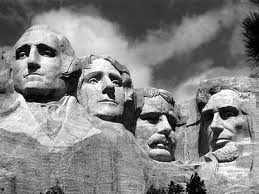
\includegraphics[width=3.6in]{Images/MtRush.png}

Here we have only one image, and we'll store it as a matrix $A$ (rows of
the matrix corresponding to rows of $A$).  we'll use NMF to compress it,
not do classification.  First obtain $A$:

\begin{lstlisting}
> library(pixmap) 
# read file
> mtr <- read.pnm('MtRush.pgm') 
> class(mtr)
[1] "pixmapGrey"
attr(,"package")
[1] "pixmap"
# mtr is an R S4 object of class "pixmapGrey"
# extract the pixels matrix
> a <- mtr@grey
\end{lstlisting}

Now, perform NMF with rank 50, find the approximation to $A$, and
display it:

\begin{lstlisting}
> aout <- nmf(a,50)
> w <- aout@fit@W
> h <- aout@fit@H
> approxa <- w %*% h
# brightness values must be in [0,1]
> approxa <- pmin(approxa,1) 
> mtrnew <- mtr
> mtrnew@grey <- approxa 
> plot(mtrnew)  # dispatched to plot.pixmapGrey()
\end{lstlisting}

Here is the result:

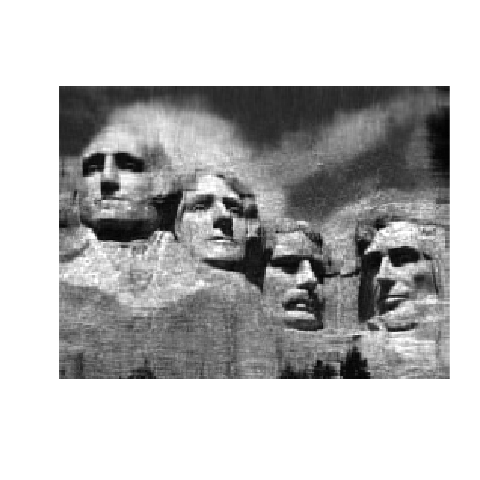
\includegraphics[width=3.6in]{Images/MtRush50.png}

This is somewhat blurry.  The original matrix has dimension $194 \times
259$, and thus presumably has rank 194.\footnote{One could check this by
finding the number of nonzero eigenvalues of $A'A$, say by running
\textbf{prcomp()}.} We've approximated the matrix by one of rank only
50.  We could use this for compression, and if we had millions of
images and this amount of blurriness were acceptable, we could take this
approach.

Actually, there are better ways to compress images, and this was just an
illustration of the effect of the reduced rank.  Getting back to our
classification context, the point is:

\begin{itemize}

\item When we use the term \textit{low-rank approximation}, it is indeed
approximate, as can be seen by the blurriness.  

\item Applying NMF or PCA/SVD to a whole collection of images, e.g.\
MNIST, further heightens this approximate nature of the process.

\item But we need to do something to avoid overfitting, i.e.\ some kind
of dimension reduction, and finding a low-rank approximation does that.

\end{itemize} 

\section{The Bias vs.\ Variance Tradeoff}

The blurriness in that second picture is really an issue of bias, as
follows.  Consider a given pixel, say in the 3rd row and 52nd column. 
That pixel's intensity in the second picture will be a weighted
average of various pixels in the first picture.  Some of the latter may
be in locations within the picture that are somewhat far away from the
3rd row and 52nd column.  This biases the pixel in the second picture.

On the other hand, there definitely is a variance issue.  Let's review
what this entails.

Recall from Chapter \ref{chap:overfit} that an intuitive way to view the
variance issue in overfitting is that our data are being ``shared'' by
the various things we're estimating, so that in a rough sense, each of
these things has less data to itself.  Less data means more
sample-to-sample variability, i.e.\ higher variance.  In linear
regression with $p$ features, we are estimating $p+1$ parameters
(including $\beta_0$); the larger $p$ is, the larger the variance of the
estimated $\beta_i$.  Thus in turn we get larger variance to our
predicted values.  For predicting a new case, different samples will
give us different predictions, and larger $p$ will give us higher
variance in our predicted value for that case.

Let $n$ and $m$ denote the number of rows and columns in $A$.  Then $W$
and $H$ will be of dimensions $n \times k$ and $k \times m$.  Well,
then, how many parameters are we estimating?  It's

\begin{equation}
nk + km = k(n+m)
\end{equation}

So, the larger we make $k$, the larger the variance.

In other words, in predicting a specific $A_{ij}$, our predicted value
$\widehat{A}_{ij}$ will experience this tradeoff:

\begin{itemize}

\item Larger $k$ means lesser bias in our estimate of $\widehat{A}_{ij}$.

\item Larger $k$ means greater variance in $\widehat{A}_{ij}$.

\end{itemize} 

\section{Computation}
\label{nmfcomp}

How are the NMF solutions found?  What is {\bf nmf()} doing internally?

Needless to say, the methods are all iterative, with one approach being
that of the Alternating Least Squares algorithm AltLS).  It's quite
intuitive, builds on our previous material and provides insight into NMF
itself.\footnote{By the way, Alt.\ Least Squares is not the default for
{\bf nmf()}.  To select it, set {\bf method = 'snmf/r'}.}

And most importantly ---  AltLS is easily adapted to the recommender
systems setting.  Remember, recommender systems differ fundamentally
from, say, the image and text classification applications cited earlier,
due to the fact that some, typically the vast majority, of elements of
the $A$ matrix are unknown.  

So let's take a look, still assuming for now that $A$ \textit{is}
competely known.


\subsection{Objective Function}

We need an {\it objective function}, a criterion to optimize, in this
case a criterion for goodness of approximation. Here we will take that
to be the {\it Frobenius} norm (Section \ref{vecnorms}),

\begin{equation}
\label{froben}
\|Q\|_2 = 
\sqrt{
\sum_{i,j} Q_{ij}^2
}
\end{equation}

So our criterion for error of approximation will be

\begin{equation}
\label{errawh}
\|A - WH\|_2
\end{equation}

So, we choose $W$ and $H$ to be 

\begin{equation}
\arg \min_{w,h} \|A - wh\|_2
\end{equation}

This measure is specified in {\bf nmf()} by setting {\bf objective =
'euclidean'}.

Note that we can write (\ref{froben}) as

\begin{equation}
\label{wholething}
\|Q\|_2 = 
\sqrt{
\sum_j \left ( \sum_i Q_{ij}^2 \right )
}
\end{equation}

This mean that if we can separately minimize that inner sum, for each
$j$, we will have minimized the entire expression (\ref{wholething}).
Our strategy will depend on this.

\subsection{Alternating Least Squares}

So, how does Alternating Least Squares work?  Suppose just for a moment
that we know the exact value of $W$, with $H$ unknown.  Then for each
$j$ we could minimize

\begin{equation}
\label{errajwhj}
\|A_{\cdot j} - W H_{\cdot j}\|_2
\end{equation}

We are seeking to find $H_{\cdot j}$ that minimizes (\ref{froben}), with
$A_{\cdot j}$ and $W$ known.  But since the Frobenius norm is just a sum
of squares, that minimization is just a least-squares problem, i.e.\
linear regression, just as in Section \ref{howmin}.  We are
``predicting'' $A_{\cdot j}$ from $W$,

So again in the notation of Section \ref{lmdetails}:

\begin{itemize}

\item The matrix $A$ there is our $W$ here, known.

\item The vector $D$ there is our $A_{\cdot j}$ here, known.

\item The vector $b$ there is our $H_{\cdot j}$ here, unknown and to be
solved for.

\end{itemize} 

So we compute

\begin{lstlisting}
> h[,j] <- lm(a[,j] ~ w - 1)$coef
\end{lstlisting}

for each $j$.\footnote{The -1 specifies that we do not want a constant term in
the model.}

On the other hand, suppose we know $H$ but not $W$.  We could take 
transposes,

\begin{equation}
A' = H' W'
\end{equation}

and then just interchange the roles of $W$ and $H$ above.  Here a call
to {\bf lm()} gives us a column of $W'$, thus a row of $W$, and we do
this for all rows.

Putting all this together, we first choose initial guesses, say random
numbers, for $W$ and $H$; {\bf nmf()} gives us various choices as to how
to do this.  Then we alternate: Compute the new guess for $W$ assuming
$H$ is correct, then choose the new guess for $H$ based on that new $W$,
and so on.

During the above process, we may generate some negative values.  If so,
we simply truncate to 0.

\subsection{Back to Recommender Systems:  Dealing with the Missing Values}

In our recommender systems setting, of course, most of $A$ is missing.
But we can easily adapt to that.  Roughly speaking, in (\ref{errajwhj}),
do these replacements:

\begin{itemize}

\item replace $A_{.j}$ by the known portion of $A_{.j}$

\item replace $W$ by the corresponding rows of $W$

\end{itemize} 

Then proceed as before.  

Here is a little example.  Say $A$ ix $5 \times 5$ and we want rank 3.
Then $W$ and $H$ are of sizes $5 \times 3$ and $3 \times5$.  

Note too that $(WH)_{.j}$, thus column $j$ of our approximation to $A$,
is a linear combination of the columns of $W$, with coefficients being
$H_{.j}$.


Suppose

\begin{equation}
A_{.4} = 
\left (
\begin{array}{r}
NA \\
3 \\
NA \\
8 \\
2
\end{array}
\right )
\end{equation}

Then in (\ref{errajwhj}) we replace $A_{.5}$ by

\begin{equation}
\label{smalla}
\left (
\begin{array}{r}
3 \\
8 \\
2 
\end{array}
\right )
\end{equation}

Also, replace $W$ by

\begin{equation}
\label{smallw}
\left (
\begin{array}{rrr}
w_{21} & w_{22} & w_{23} \\
w_{41} & w_{42} & w_{43} \\
w_{51} & w_{52} & w_{53} \\
\end{array}
\right )
\end{equation}

Remember, at this stage, $W$ is assumed known.  So, we just use
\textbf{lm()}, ``predicting'' (\ref{smalla}) from (\ref{smallw}) to find
$h_{.4}$.


% \subsubsection{Multiplicative Update}
% 
% Alternating Least Squares is appealing in several senses.  At each
% iteration, it is minimizing a {\it convex} function, meaning in essence
% that there is a unique local and global minimum; it is easy to
% implement, since there are many least-squares routines publicly
% available, such as {\bf lm()} here; and above all, it has a nice
% interpretation, predicting columns of $A$.
% 
% Another popular algorithm is {\it multiplicative update}, due to Lee and
% Seung.  Here are the update formulas for $W$ given $H$ and {\it vice
% versa}:
% 
% \begin{equation}
% W \leftarrow W \circ 
% \frac
% {AH'}
% {WHH'}
% \end{equation}
% 
% \begin{equation}
% H \leftarrow H \circ 
% \frac
% {W'A}
% {W'WH}
% \end{equation}
% 
% where $Q \circ R$ and $\frac{Q}{R}$ represent \underline{elementwise}
% multiplication and division with conformable matrices $Q$ and $R$, and
% the juxtaposition $QR$ means ordinary matrix multiplication.

\subsection{Convergence and Uniqueness Issues}

There are no panaceas for applications considered here.  Every solution
has potential problems.  I like to call this the Pillow Theorem ---
pound down on one fluffy part and another part pops up.

Unlike the PCA case, one issue with NMF is uniqueness --- there might
not be a unique pair $(W,H)$ that minimizes (\ref{errawh}).  In fact,
one can see this immediately:  Doubling $W$ while having $H$ leaves the
product $WH$ unchanged.  Of course, the product is all that really
counts, but in turn, this may result in convergence problems. The NMF
documentation recommends running {\bf nmf()} multiple times; it will use
a different seed for the random initial values each time.

The Alternating Least Squares method used here is considered by some to
have better convergence properties, since the solution at each iteration
is unique.  This may come at the expense of slower convergence.

\section{How Do We Choose the Rank?}
\label{chooserank}

This is not an easy question.  One approach would be to use
\textbf{prcomp}, or for that matter \textbf{svd()}, to find the
eigenvalues, then take our rank to be the number of ``large''
eigenvalues, as discussed in Chapter \ref{chap:linalg}.  

Of course, the typical way rank is chosen is cross validation.

\section{Why Nonnegative?}

In the applications we've mentioned here, we always have $A_{ij} \geq 0$.
However, that doesn't necesarily mean that we need $W$ and $H$ to be
nonnegative, and indeed if we were to use PCA, they may not so.  (With
PCA, even their product could have negative element, which we would
truncate to 0.)  Why use NMF, i.e.\ why insist that the factors $W$ and
$H$ themselves be nonnegative?

There are a couple of reasons NMF may be preferable.  First, truncation
may be questionable if we have a lot of negative values.  But the second
reason is that NMF may be more useful, as follows:

In a facial image recognition case, say, there is hope that the vectors
$W_{\cdot j}$ will be {\it sparse}, i.e.\ mostly 0s. Then we might have,
say, the nonzero elements of $W_{\cdot 1}$ correspond to eyes, $W_{\cdot
2}$ correspond to nose and so on with other parts of the face.  We are
then ``summing'' to form a complete face.  This may enable effective
{\it parts-based recognition}, with helpful interpretations.

In our recommender systems setting, this parts-based effect, NMF would
give us crisper distinction among the various synthetic users.  This may
reveal clusters of user behavior, which could be quite helpful to the
analyst.

Another point is that the nonnegativity allows us to better fulfill the
``synthetic users'' idea from Section \ref{synth}.  To make these more
realistic, they should be on the same level as real user ratings.  We
can arrange this by simply scaling down each $H_{i.}$ to the ratings
scale, e.g. 1 to 5 for the MovieLens data.  

% \section{Functions in rectools}
% 
% The \textbf{recoSystem} package by Chih-Jen Li \textit{et al} has a good
% implementation of NMF for recommender systems (i.e.\ it handles the
% missing values).  However, it uses R6 classes (and is complicated in
% other ways), which are unfamiliar to many R users, so the
% \textbf{rectools} package provides wrappers.  Basic call forms are:
% 
% \begin{lstlisting}
% trainReco(ratingsIn,rnk=10,nmf=FALSE)
% predict.RecoS3(recoObj,testSet)
% \end{lstlisting}
% 
% Here \textbf{ratingsIn} is the usual three-column (userID,itemID,rating)
% (plus covariates, if any) data frame; \textbf{rnk} is the desired rank;
% \textbf{nmf} is false for SVD, true for NMF; \textbf{recoObj} is the 
% return value from \textbf{trainReco()}; and \textbf{testSet} is the test
% set, in the same format as \textbf{ratingsIn}, minus the ratings column.
% 
% The return value from \textbf{trainReco()} is an R S3 object of class
% 'RecoS3', with components $P$ and $Q$, corresponding to $W$ and $H'$ in
% our notation.  In the case of covariates (see below), some R
% \textbf{attributes} are also included.

\section{``Bias'' Removal}

As noted in Chapter \ref{chap:knn}, some users tend to give more liberal
ratings, while others tend to be more cautious.  Similarly, some items
tend to be rated more highly than others.  One way of dealing with
that is to adjust our ratings matrix $A$ accordingly:  For each user
$i$, let $R_i$ denote the average of all known ratings from that user.
Also, for each item $j$ let $S_j$ denote the average of all known ratings
for that item.  These are termed \textit{biases}. Then do the replacement

\begin{equation}
A_{uv} \leftarrow A_{uv} - R_u - S_v
\end{equation}

and then form the matrix factorization as usual.  In the end, after
estimating the unknown entries in $A$, restore
the subtracted quantities:

\begin{equation}
A_{uv} \leftarrow A_{uv} + R_u + S_v
\end{equation}

\section{Dealing with Covariates}

Why stop with just removing ``biases''?  We can go a step further and
account for user or item covariates.

The easiest approach to handling covariates is to simply ``subtract them
out'' for the data via linear regression, then run NMF/SVD on the
resulting \textit{residuals},\footnote{In regression modeling, the
values of true Y minus the fitted model are called ``residuals.'' They
are often used to assess quality of model fit. There is a
\textbf{residuals}} component in the S3 object returned by
\textbf{lm().} and finally, at the prediction stage, add the regression
values back in.

Here are relevant code excerpts:

\textbf{trainReco()}:

\begin{lstlisting}
hasCovs <- (ncol(ratingsIn) > 3)
if (hasCovs) {
    covs <- as.matrix(ratingsIn[, -(1:3)])
    lmout <- lm(ratingsIn[, 3] ~ covs)
    # now make fake ratings; for NMF, must be >= 0
    minResid <- min(lmout$residuals)  
    ratingsIn[, 3] <- lmout$residuals - minResid
}
...
r$train(train_set, opts = list(dim = rnk, nmf = nmf))
result <- r$output(out_memory(), out_memory())
attr(result, "hasCovs") <- hasCovs
if (hasCovs) {
    attr(result, "covCoefs") <- coef(lmout)
    # add the residuals back in
    attr(result, "minResid") <- minResid
}
class(result) <- "RecoS3"
result
\end{lstlisting}

\textbf{predict.RecoS3()}:

\begin{lstlisting}
if (hasCovs) {
     tmp <- c(1, testCovs[i, ]) %*% covCoefs + minResid
}
pred[i] <- p[j, ] %*% q[k, ] + tmp
\end{lstlisting}

In the covariates case, \textbf{trainReco()} replaces the ratings by the
residuals, so the product $WH$ approximates them rather than the
original $A$.  Then in \textbf{predict.RecoS3()}, after multiplying
$W_{i \cdot}$ and $H_{\cdot j}$, the estimated regression function value
for the given case is added back in.

The role of \textbf{minResid} is this:  If we are using NMF, fitting to the
residuals, which are both positive and negative, makes no sense.  So, we
subtract the (algebraically) smallest residual, resulting in only
nonnegative values.  Again, this is added back in later on.

\section{Regularization}

Recall Section \ref{dosomething}, where we introduced the idea of
shrinkage as a guard against overfitting.

For NMF (or SVD), we probably don't want to force some predicted ratings
to 0, the $l_2$ norm is a popular choice.  Thus, instead of choosing $W$ and
$H$ to minimize (\ref{errawh}), we minimize

\begin{equation}
||A - WH||_2 + \gamma_1 ||W||_2^2 + \gamma_2 ||H||_2^2
\end{equation}

Both $\gamma_1$ and $\gamma_2$ are tuning parameters.

The \textbf{NMF} package offers regularization as an option.

\section{The recosystem Package}

The \textbf{recosystem} package does matrix factorization specifically
for recommender systems, i.e.\ specifically for settings in which the
matrix $A$ has many missing values.  It's written by experts in
numerical matrix factorization, and features a number of useful options.

Below is a \textbf{recosystem} session using the small MovieLens data.
Let's suppose we've already decided on rank $k = 20$, say by cross
validation, and now we'll go back to using the full dataset for our
predictions.

\begin{lstlisting}
> library(recosystem)
# all action will take place within r;
# typically the output of a function will be stored as a new component in r
> r <- Reco()
> ml <- read.table('u.data',header=F)
# need to create an object of class 'DataSource', specifying which
# columns are user IDs, item IDs and ratings
> ml.dm <- data_memory(ml[,1],ml[,2],ml[,3],index1=TRUE)
\end{lstlisting}

\begin{lstlisting}
# do the factorization, with rank 20; do use NMF
> r$train(ml.dm,opts=list(dim=20,nmf=TRUE))
iter      tr_rmse          obj
   0       2.0381   5.0056e+05
   1       1.0296   1.7402e+05
   2       0.9529   1.6028e+05
   3       0.9449   1.5868e+05
   4       0.9418   1.5811e+05
   5       0.9397   1.5774e+05
   6       0.9382   1.5749e+05
   7       0.9371   1.5729e+05
   8       0.9362   1.5713e+05
   9       0.9355   1.5701e+05
  10       0.9348   1.5690e+05
  11       0.9343   1.5681e+05
  12       0.9338   1.5673e+05
  13       0.9334   1.5666e+05
  14       0.9330   1.5660e+05
  15       0.9327   1.5654e+05
  16       0.9324   1.5649e+05
  17       0.9321   1.5645e+05
  18       0.9318   1.5641e+05
  19       0.9316   1.5637e+05
# training went for 20 iterations; RMSE is the square root
#    of mean squared error
# for large data, write to disk, otherwise in memory
> result <- r$output(out_memory(),out_memory())
> str(result)
List of 2
 $ P: num [1:943, 1:20] 0.676 0.677 0.574 0.836 0.574 ...
 $ Q: num [1:1682, 1:20] 0.712 0.614 0.568 0.645 0.612 ...
# P and Q are W and H'
> w <- result$P
> h <- t(result$Q)
# let's try a prediction, with a known rating
> head(ml)
   V1  V2 V3        V4
1 196 242  3 881250949
2 186 302  3 891717742
3  22 377  1 878887116
...
> w[22,] %*% h[,377]
         [,1]
[1,] 2.196976
# or just have recosystem do it for us
> preds <- r$predict(ml.dm,out_memory())
> head(preds)
[1] 3.979107 4.212397 2.196976 3.601082 3.900878 4.467487
\end{lstlisting}

\section{How Do We Minimize (\ref{slh})?}
\label{howmin}

The answer, as it was in Section \ref{nmfcomp}, is to convert the
question to one of linear regresson.

It will be helpful to keep some concrete numbers in mind, say with the
MNIST data.  Say we wish a rank of 50.  Then

\begin{itemize}

\item $A$ is 70000x784;

\item $W$ is 70000x50;

\item $H$ is 50x784;

\item $S$ is 1x784; and

\item $l$ is 50x1.

\end{itemize} 

Keeping these numbers in mind as concrete examples,
now note that in (\ref{slh}),

\begin{equation}
\label{slh1}
|| S - l'H ||^2 = (S - l'H)(S - l'H)'
\end{equation}

This looks pretty close to (\ref{dab}).  But recall that $S$ and $l'H$
are row vectors, so (\ref{slh1}) looks slightly different.  Now, using
the fact from linear algebra that $(UV)' = V'U'$, (\ref{slh1}) says

\begin{equation}
\label{slh2}
|| S - l'H ||^2 = (S' - H'l)(S' - H'l)
\end{equation}

Now it's in the form of (\ref{dab}), so our minimization problem is
solved!  In (\ref{famouslm}), just set $D$, $A$ and $b$ to $S'$, $H'$
and $l$, respectively.  This gives us

\begin{equation}
\lambda = (HH')^{-1} HS'
\end{equation}

We could compute this directly, using R's matrix operations (for matrix
inversion, we can use \textbf{solve()}, or for better numerical
accuracy, \textbf{solve.qr()}), but it's easier to send it to
\textbf{lm()}, e.g.

\begin{lstlisting}
lm(s ~ t(h) - 1)$coef
\end{lstlisting}

Again, the `-1'' tells \textbf{lm()}, ``Don't add a column of 1s to $H'$.''
